\chapter{Sensoren}
\renewcommand{\kapitelautor}{Autor: Lucas Ullrich}

%%%%%%%%%%%%%%%%%%%%%%%%%%%%%%%%%%%%%%%%%%%%%%%%%%%%%%%%%%%%%%%%%%%%%%%%%%%%%%%
\section{Pixy CMUcam5}
Bei der PIXY CMUcam5 handelt es sich um ein Open Source Kameramodul, welches über eine Objekterkennung verfügt. Mit diesem ist es möglich sogenannte Colorcodes oder einfache Objekte zu erkennen.

\begin{figure}[H]
  \begin{centering}
    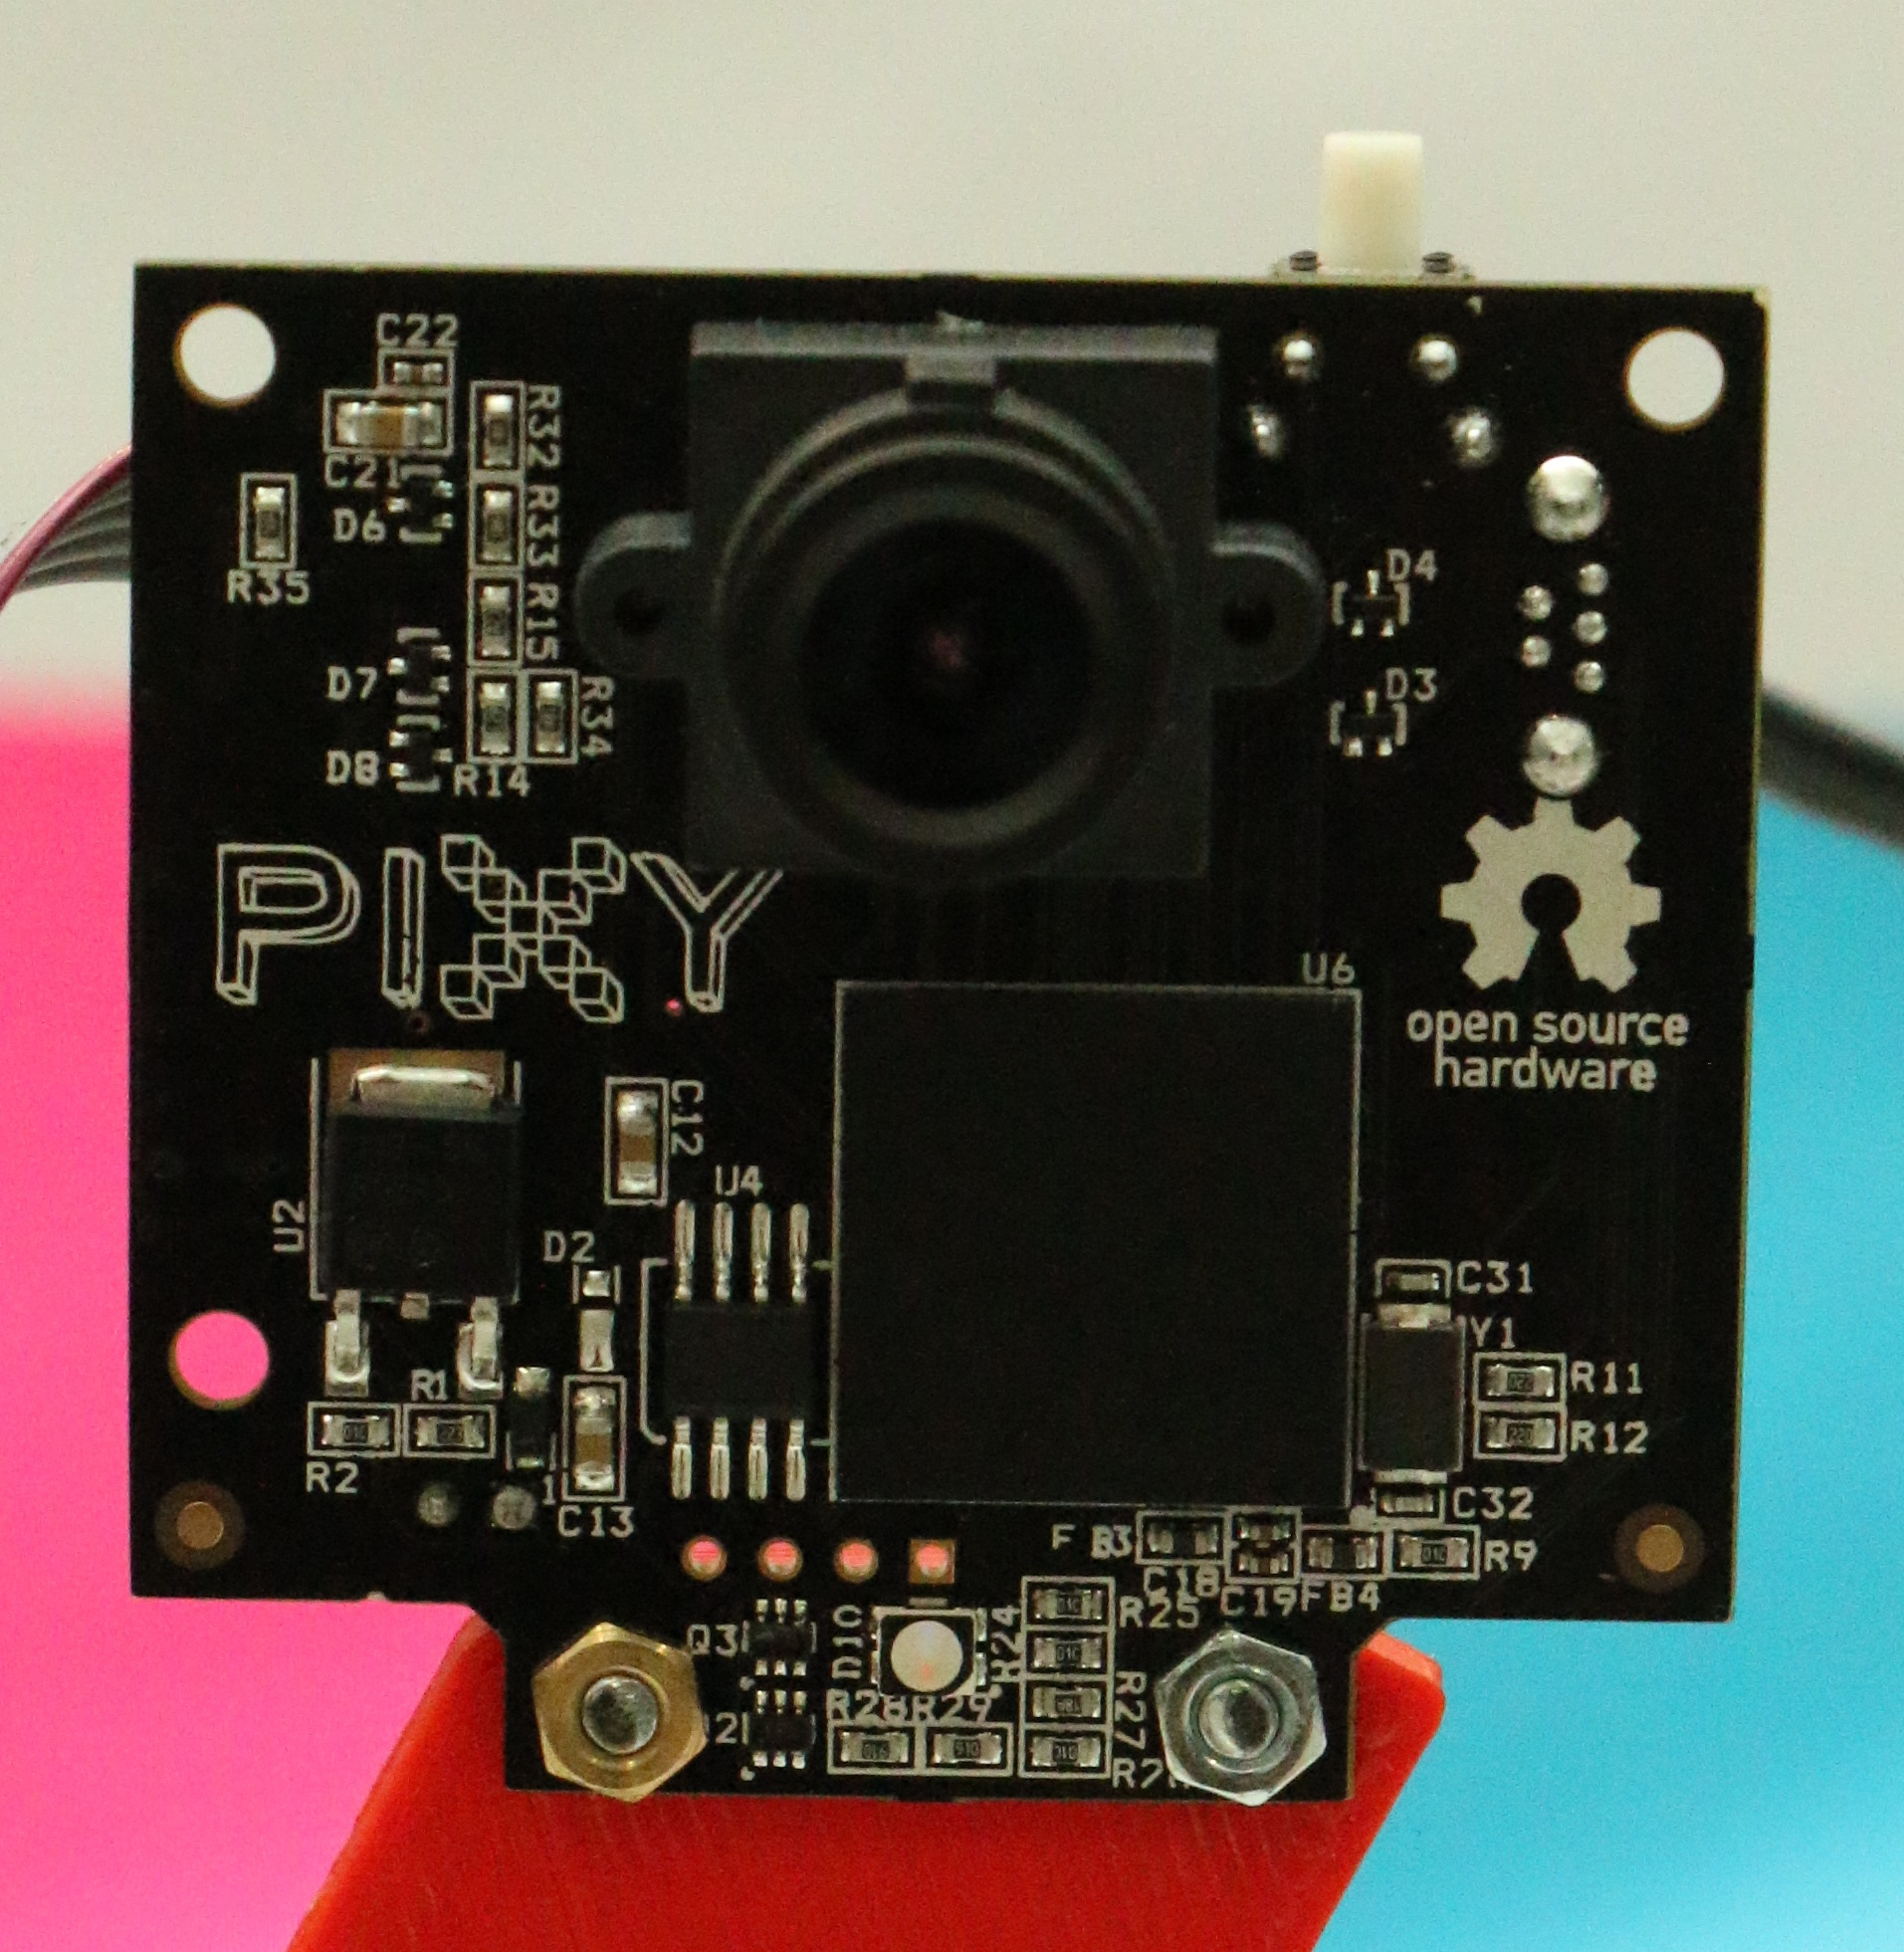
\includegraphics[width = 0.4\textwidth]{Bilder/Pixy_CMUcam5}
  \par\end{centering}
  \caption{PIXY CMUcam5}
  \label{PIXY}
\end{figure}

\begin{figure}[H]
  \begin{centering}
    \subfigure[Colorcode]{
\includegraphics[width = 0.4\textwidth]{Bilder/Colorcode}}
    \subfigure[Objekt]{
\includegraphics[width = 0.4\textwidth]{Bilder/Colorcode}} %%%%%%%%%Objekt statt Colorcode
  \par\end{centering}
  \caption{Erkennbare Objekttypen}
  \label{PIXY_Objekte}
\end{figure}

  \subsection{Technische Planung}
    \subsubsection{Mögliche Verfahren zur Positionserkennung}
    Hier muss grundsätzlich zwischen zwei Messmethoden unterschieden werden:
    \begin{itemize}
      \item Absolute Positionsmessung
      \item Relative Positionsmessung
    \end{itemize}
    \paragraph{Absolute Positionsmessung}
    Hier wird die Postion von einem gleichbleibenden Punkt aus gemessen. Dabei ist ein konstanter Referenzpunkt wichtig. Verändert sich der Referenzpunkt oder kann die Distanz zu diesem nicht genau gemessen werden ist die Messung unbrauchbar.
    Für eine absolute Positionsmessung bieten sich diverse Triangulationsverfahren an, diese sind ausgesprochen rechenaufwändig und benötigen meist eine sehr genaue Laufzeitmessung. Für die Triangulation können die unterschiedlichsten Signale verwendet werden, am gängigsten sind jedoch jene die mit elektromagnetischen Wellen arbeiten, \zB WLAN, Bluetooth. Die bedeutet, dass sich die Signale mit Lichtgeschwindigkeit ausbreiten.
    Für eine Messung derart schneller Signale muss ein hoher Aufwand betrieben werden um eine Messgenauigkeit von einigen cm zu erzielen.

    \paragraph{Relative Positionsmessung}

  \subsection{Umsetzung}

    \subsubsection{SPI Schnittstelle}

    \subsubsection{Erkennen und auswerten eines Bildes}

  \subsection{Herausforderungen und Lösungen}

%%%%%%%%%%%%%%%%%%%%%%%%%%%%%%%%%%%%%%%%%%%%%%%%%%%%%%%%%%%%%%%%%%%%%%%%%%%%%%%
\section{Ultraschall}

  \subsection{Technische Planung}

  \subsection{Umsetzung}

    \subsubsection{Bestimmen der Flughöhe}

  \subsection{Herausforderungen und Lösungen}

\chapter{Aktoren}
\renewcommand{\kapitelautor}{Autor: Lucas Ullrich}

%%%%%%%%%%%%%%%%%%%%%%%%%%%%%%%%%%%%%%%%%%%%%%%%%%%%%%%%%%%%%%%%%%%%%%%%%%%%%%%
\section{Propeller, A E T und R}

  \subsection{Technische Planung}

  \subsection{Umsetzung}

  \subsection{Herausforderungen und Lösungen}
